Nesse capítulo serão realizados os laboratórios 7, 8, 9 e 10. Mais algumas
aplicações em biologia são desenvolvidas.

\begin{enumerate}[label=\textbf{Lab \arabic*:}]
    \setcounter{enumi}{6}

    \item Modelo para Epidemia 
    
    Nesse laboratório, um simples modelo compartimental SEIR é desenvolvido
    segundo a figura \ref{fig1:seir}. Um controle de vacinação é visualizado
    como  efeito. É uma simplificação que permite tirar conclusões similares
    àquelas obtidas pela comunidade científica. 

    \begin{figure}[hb]
        \center
        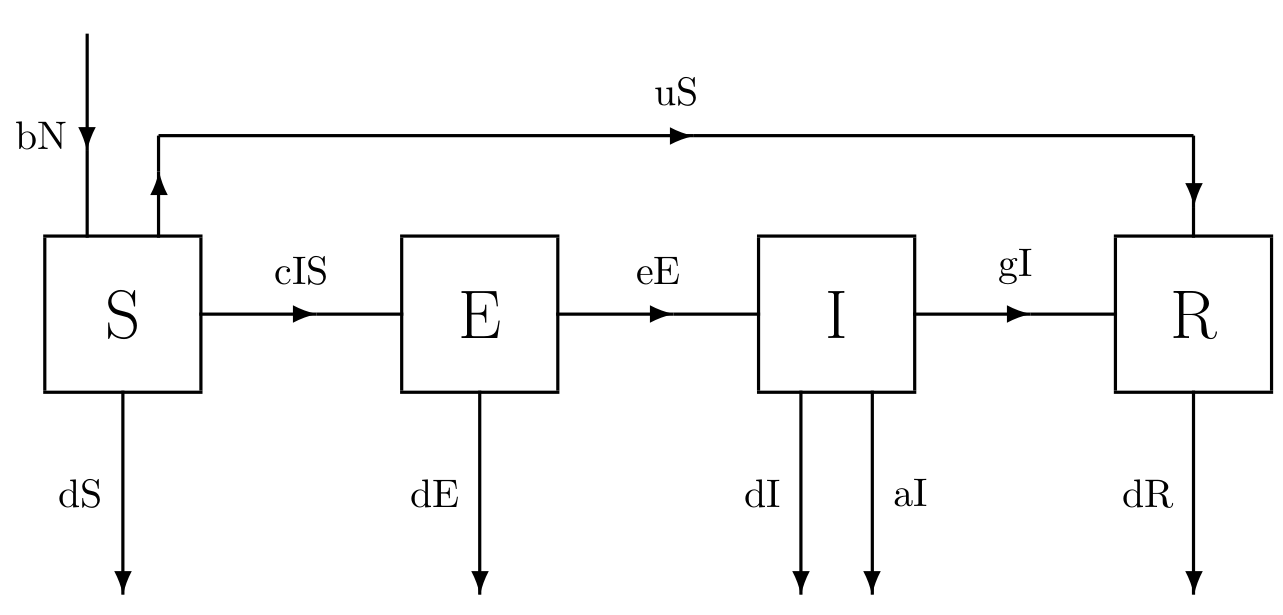
\includegraphics[width = \textwidth]{../images/flow-chat-seir.png}
        \caption{O gráfico de fluxo do modelo é explicado aqui.}
        \label{fig1:seir}
    \end{figure}

    \item Câncer
    
    Modelo do tratamento de células cancerosas por quimioterapia, com objetivo
    de minimizar os efeitos negativos do uso das drogas, mas também minimizar
    a densidade dessas células no corpo. É simplificado, porém apresenta dois
    componentes importantes: o crescimento Gompertzian e a hipótese de Skipper
    para a morte das células segundo o uso das drogas. 

    \item Colheita de peixe  
    
    Uma população de peixes é inserida em um tanque e é deixada para ser
    caçada, com morte natural, mas sem taxa de nascimento. Queremos maximizar
    a massa de peixes caçada, enquanto minimizamos o gasto com a colheita.
    Restrições são consideradas. 
 
\end{enumerate}